\chapter{DEA} \label{CAP:uno}
\section{Introduzione}
\bigskip

\paragraph{} Il \emph{Data Envelopment Analysis}, che indicheremo con l'acronimo \emph{DEA}, \`e un metodo non parametrico per la stima delle frontiere di efficienza. \`E usato per misurare empiricamente l'efficienza produttiva delle unit\`a decisionali, \emph{DMU} (Decision Making Units). Gli approcci non parametrici hanno il vantaggio di non assumere particolari forme alla frontiera, ma non forniscono una relazione generale tra input e output.
\paragraph{} Per introdurci allo studio della DEA, iniziamo con l'esporre un primo esempio esplicativo. Supponiamo di avere otto negozi $\{A,\cdots,H\}$, ciascuno dei quali dispone di un certo numero di impiegati e produce un certo quantitativo di vendite (quest'ultime in scala 1:100000). Una semplice misura di efficienza per ciascun negozio può essere espressa dalla seguente formula:
\begin{equation}
\dfrac{Output}{Input}
\end{equation}
dove le vendite sono gli output e gli impiegati l'input. Mostriamo in \autoref{TAB:SiSo} i dati relativi al problema precedentemente esposto.

\begin{table}[H]
\centering
\begin{tabular}{lccccccccc}
\hline 
Negozio & A & B & C & D & E & F & G & H \\ 
\hline 
Impiegato & 2 & 3 & 3 & 4 & 5 & 5 & 6 & 8 \\ 
\hline 
Vendita & 1 & 3 & 2 & 3 & 4 & 2 & 3 & 5 \\ 
\hline 
Vendita/Impiegato & 0.5 & 1 & 0.667 & 0.75 & 0.8 & 0.4 & 0.5 & 0.625 \\ 
\hline 
\end{tabular}
\caption{Esempio con singolo input e singolo output} \label{TAB:SiSo}
\end{table}

\paragraph{} Analizzando i coefficienti contenuti nell'ultima riga della \autoref{TAB:SiSo}, possiamo identificare B come negozio pi\`u efficiente. Si pu\`o rappresentare graficamente questa situazione, mettendo sulle ascisse il numero di impiegati e sulle ordinate le vendite, come in \autoref{FIG:SiSo}.

\begin{figure}[H]
\centering
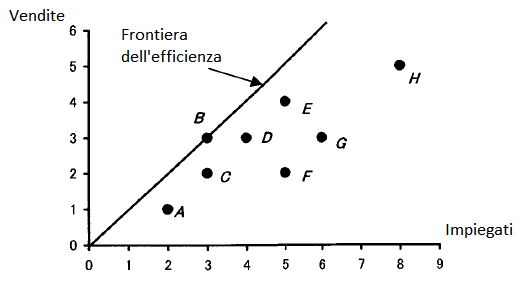
\includegraphics[scale=1]{Img/GraficoSISO.png}
\caption{Rappresentazione grafica dell'esempio}\label{FIG:SiSo}
\end{figure}

\paragraph{}Osserviamo dalla \autoref{FIG:SiSo} che per ogni negozio possiamo esprimere le vendite di ciascun dipendente come coefficiente angolare della retta che congiunge il punto del grafico corrispondente al negozio con l'origine. La retta con la pendenza maggiore (in questo caso quella passante per B) viene chiamata \emph{Frontiera dell'efficienza}. La scelta del nome \`e dovuta al fatto che i punti del grafico non posso trovarsi al di sopra di questa retta.

\paragraph{} Proseguiamo l'analisi dell'esempio valutando l'efficienza di tutti i negozi rispetto a B, con la formula
\begin{equation}\label{EQ:siso}
0\leq \dfrac{\text{Vendite per impiegato del negozio i-esimo}}{\text{Vendite per impiegato di B}} \leq 1
\end{equation}
ottenendo:
\begin{table}[H]
\centering
\begin{tabular}{lccccccccc}
\hline 
Negozio & A & B & C & D & E & F & G & H \\ 
\hline 
Efficienza & 0.5 & 1 & 0.667 & 0.75 & 0.8 & 0.4 & 0.5 & 0.625 \\ 
\hline 
\end{tabular}
\caption{Esempio con singolo input e singolo output} \label{TAB:SiSoContratta}
\end{table}

\paragraph{} A questo punto possiamo proporre delle strategia per rendere efficienti i negozi inefficienti: graficamente si traduce nell'avvicinare i punti rappresentanti i negozi alla frontiera dell'efficienza. Per esempio, il negozio A, pu\`o essere migliorato:
\begin{align}
&\text{riducendo l'input (numero di impiegati)}\label{EQ:input oriented}\\
&\text{aumentando l'output (vendite)}\label{EQ:output oriented}
\end{align}
Le due alternative proposte equivalgono rispettivamente ai punti $A_1$ e $A_2$ riportati in \autoref{FIG:SiSoNegozioA}: il punto $A_1$ corrisponde alla situazione in cui si riducono gli impiegati da 2 a 1, mantenendo le vendite inalterate; il punto $A_2$ invece, corrisponde ad un aumento delle vendite da 1 a 2 lasciando inalterato il numero di impiegati. Infine, tutti gli altri punti del segmento $\overline{A_1A_2}$ rappresentano un miglioramento del negozio A non ottenibile tramite le opzioni (\ref{EQ:input oriented}) o (\ref{EQ:output oriented}).

\begin{figure}[H]
\centering
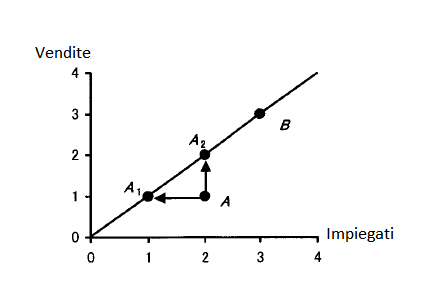
\includegraphics[scale=1]{Img/GraficoSiSoNegozioA.png}
\caption{Miglioramento del negozio A}\label{FIG:SiSoNegozioA}
\end{figure}

\begin{oss}
Il nome 'Data Envelopement Analysis' proviene dalla propriet\`a della frontiera dell'efficienza che avvolge (\emph{envelope}) tutte le rappresentazioni grafiche delle DMU.
\end{oss}
Non è ragionevole ritenere che la frontiera dell'efficienza si estenda all'infinito con la stessa pendenza. Analizzeremo questo problema in seguito utilizzando diversi modelli DEA. Tuttavia, diamo per scontato che questa linea è efficace nel range di interesse e chiamiamo tale assunzione 'rendimenti di scala costanti'.